\documentclass{article}
\usepackage{graphicx} % Required for inserting images
\usepackage[utf8]{inputenc}
\usepackage[T1]{fontenc}
\usepackage[spanish, mexico]{babel}
\usepackage{amsmath}
\usepackage{amssymb}
\usepackage{enumitem}
\usepackage{geometry}
\usepackage{url}
\usepackage{float}
\geometry{margin=2.5cm}

\title{Modelado y Programación\\
Reporte del Proyecto 1}
\author{Profesor: Canek Peláez Valdés\\
Alumno: Angel Antonio Martínez Méndez}

\date{September 2026}

\begin{document}

\maketitle

\section*{Resumen}

El primer proyecto de la materia de Modelado y Programación se trata de un chat grupal con diferentes funcionalidades, a saber: mandar mensajes públicos, privados, consultar la lista de usuarios, cambiar de estado y crear cuartos. En este reporte, se incluye una introducción al proyecto, la parte del análisis y diseño realizado, la implementación del mismo y nuestras conclusiones al terminarlo.\\

\section*{Introducción}
Una herramienta moderna muy común, al menos hoy en día, para la comunicación entre individuos, que se da a través de la red, es la capacidad de chatear con otras personas al readedor de todo el mundo. Ya sea en foros, servicios de mensajería, redes sociales e inclusive con la IA, es escencial poder mantener una conversación escrita para cumplir con todos estos fines.\\

De aquí que, como primer proyecto para la materia de Modelado y Programación, se nos haya encomendando realizar un chat grupal, el cual es bastante útil y enriquecedor como programador saber cómo funcionan y, en consecuncia, poder implementar al menos una versión de juguete de estos. Pues es un agujero de conejo que te introduce a muchos conceptos importantes sobre el diseño de este tipo de programas y lo complejos que pueden llegar a ser.\\

Para esta tarea, solo se nos dió un procotocolo de transmisión de información (TCP); el cual es el esqueleto de todo el programa. El protocolo es básicamente una serie de reglas deben seguir los programas o dispositivos que requieren de un intercabio de datos efectivo. De esta forma, es posible agrupar la información para que llegue con un orden y de forma estructurada de un punto a otro.\\

El TCP es la estructura que utiliza el internet para recibir y enviar datos cuando existen miles de solicitudes por parte de dispositivos al rededor del mundo. Y un chat, es solo una instancia particular que surge como parte de este sofisticado mecánismo.\\

Los principales protagonistas de nuestro chat son: el servidor y el cliente. El servidor, es un programa el cual será el responsable de mantener un orden en la información que van a recibir nuestros usuarios finales con ayuda del protocolo. El cliente, es el programa que van a ejecutar los usuarios para comunicarse con otros que estén usando el mismo servidor. De aquí, que solo hay un servidor y múltiples clientes.\\

Hasta ahora la idea parece sencilla, pero es aquí donde se empieza a complicar el asunto, debido a que hay muchos entes detrás de estos dos programas que logran comunicación entre dos personas. Lo cual da pauta a la sección.

\section*{Análisis y diseño}

Cómo mencionamos, nuestro programa pricipal, el chat, esta conformado por dos subprogramas los cuales van a trabajar en conjunto para poder lograr nuestro objetivo; poder comunicar a dos personas a distancia. Ambos, tienen comportamientos y atributos distintos. Es por ello, que lo más natural para poder trabajar con estos es la orientación a objetos (POO).\\

Además, conviene usar un patrón de diseño para hacer más manejable y tener un orden en nuestro futuro código al implementar la solución de este programa. En este caso, usaremos el Modelo-Vista-Controlador (MVC), que nos permitira tener un espacio para cada componente de la solución de este problema. Una parte para la lógica, otra para tener aquellos entes auxiliares que van a usar ambos programas y la vista, que en nuestro caso es la terminal.\\

De esta manera, nuestro análisis inicia con el protocolo. Que en realidad, es la parte más sencilla abarcar. Aunque como mencionábamos, es también el esqueleto de nuestro programa, pues dictamina todas las funcionalidades que tiene el mismo y los posibles estados en los que puede caer cuando un usuario lo utiliza. De aquí que una enumeración pueda maneajor todos los datos que ofrece el protocolo. \\

Y como todo buen programa que pueden usar muchas personas, necesita un ente que regule todo lo que ocurre en él. Es aquí, donde entra el trabajo del servidor. El cual, es la parte más complicada y podría decirse que el corazón de nuestro programa. Como es un objeto regulador, va a necesitar de herramientas que verifiquen la información que va a recibir. Los datos que tienen sentido, los marca el protocolo, pero la forma en que va a organizar la información de los distintos usuarios, es harina de otro costal.\\

Además, solo debe haber una instancia común del servidor el cual todos los usuarios interesados en comunicarse deberán acceder para mantener una conversación. Esto es sencillo de resolver si usamos el concepto de IP y puerto. Una dirreción IP identifica de forma única un dispositivo en la red, justo ese dispositivo será la computadora que ejecute al servidor. Y un puerto identifica una aplicación o servicio específico dentro de dicho dispositivo. La aplicación será el servidor. Así, la combinación de estos dos conceptos es lo que conocemos como enchufe (socket), que será el tunel por el que pase la información de un cliente al servidor.\\

Ahora bien, el servidor debe tener la capacidad de manejar uno o varios clientes al mismo tiempo, de aquí es evidente, aunque en su momento no lo fue, que es necesaria una clase que se encargue de organizar la información que sale de cada cliente cuando estos quieran comunicarse con alguien más. Con ello, podemos hacer otra clase usuario que contenga un identificador del mismo, un enchufe para comunicarse con el manejador y su estatus; funcionalidad dada por el protocolo.\\

De este modo, cuando un cliente quiera verificarse al ejecutar la clase cliente, lo cual es necesario para evitar usuarios duplicados y que entre ruido al servidor, vamos a encapsular un manejador con un la información del cliente dada por la clase usuario. Así, también podemos verificar que el usuario no meta información extraña al servidor y, a su vez, saber que es justo ese usuario el que mando un mensaje. Lo que facilita hacer un verificador de dicho mensaje.\\

Con lo anteriormente dicho, surge la necesidad de tener una clase que cheque la serie de comandos que el cliente puede usar para poder aprovechar las funcionalides que proveé el protocolo, como: cambiar su estatus, mandar mensajes públicos y privados, desconectarse, ver quienes están conectados, crear cuartos, invitar personas a dichos cuartos, etc. Esta clase puede tener un nombre como comandos, o alguna nombre que ligue su funcionalidad con el cliente.\\

Este proceso facilita bastante el trabajo al manejador, pues este simplemente se encarga de verificar que los mensajes que recibe sean efectivamente parte del protocolo, ya no necesita verificar comandos del cliente, sino de enviar mensajes a los clientes y al propio servidor de toda la información que se esta transmitiendo. Y de aquí, esta clase puede validar estados del protocolo y mandar las respectivas respuestas a quien corresponda de una forma determinista. \\

Por lo cual, es sensato que los atributos de la clase manejador sean: un enchufe entre el servidor y el cliente, el nombre del usuario registrado y un estado compartido de datos entre otros clientes, que puede ser una estructura de datos. Aunque, si dejamos así esta clase puede que este algo incompleta, pues no hay nadie que verifique si un mensaje esta bien escrito y que el servidor sea capaz de evaluarlo sin caer en un estado indefinido.\\

Con ello, podemos mencionar algunas clases que van a ser de utilidad para el manejador, como un traductor que tome un mensaje dado ya sea por el cliente o el servidor, lo encapsule en una serie de bytes que tengan sentido en base a las reglas del protocolo, y tenga la capacidad de serializar y deserializar dicha información. Una clase estado, solo para mantener un objeto vivo con los datos compartidos de los usuarios. Y una clase cuarto, que como atributos puede tener el nombre del mismo, una estructura de datos para sus miembros y quizá otra para los invitados.\\

De aquí, que el servidor como clase ejecutable, le pida a quien instacie el servidor, la dirreción IP y el puerto que la computadora debe usar para transimitir y recibir datos de los clientes, los cuales, si se verifican de forma correcta, se le dará un hilo de ejecución, un manejador y, todos los métodos que requieran de información compartida para su funcionamiento, deberán soportar la cocurrencia que es trabajar con tantos clientes a la vez.\\

Un hilo de ejecución es básicamente la unidad de procesamiento más pequeña que tiene la computadora y los necesitamos porque son perfectos para proyectos que utilizan concurrencia, como el nuestro, y además de que tiene la capacidad de compartir información con otros hilos, en este caso se comparte la estructura de datos que sirve como un registro de todos los clientes que estan conectados al servidor.\\

Finalemente, solo falta hablar del cliente como clase ejecutable, que pide a aquel que lo ejecute la dirrección IP en la que se encuentra el dispositivo que ejecuta al servidor en una red compartida, y el puerto al que debe conectarse para encontrar al propio servidor. De esta forma, si los datos son correctos, manda a llamar una instancia de la clase comandos o bien cliente, que contiene la base por la que va a poder comunicarse con el servidor, y de aquí se encapsula a un manejador, que va a ser la instancia a la que va a pertenecer un cliente verificado y listo para comunicarse con otros en el servidor.\\

De esta manera, el usuario final no hace más que ponerse un nombre para identificarse en el chat, tiene una serie de funcionalidades en el mismo, que incluyen comunicarse con otros, ya sea con todos o con un grupo reducido de otros usuarios mediante la creación de cuartos, y jamás se entera de la lógica que hay detrás de todo lo que hace, solo sabe que existen comandos, otros usuarios y su necesidad de comunicación se ve satisfecha.\\

\section*{Implementación}

Cómo parte de nuestro análisis, mencionamos que era conveniente usar la Orientación a Objetos para la resolución de nuestro programa. Así que, necesitamos un lenguaje de programación que al menos tenga integrado este paradigma. Entonces, en nuestro caso utilizamos, Rust, como herramienta principal para códificar nuestra solución y crear el chat.\\

La razón de nuestra elección se basa principalmente en que Rust es un lenguaje de programación que posee un compilador muy robusto, que en cierta forma te enseña buenas prácticas para trabajar con la memoria sin necesitar de un recolector de basura. Cosa que no sucede en Java, lenguaje en el que estamos más familiarizados y que es puramente orientado a objetos, a diferencia de Rust que es multiparadigma.\\

La idea es que en un futuro podamos usar la experiencia que ofrece Rust para adentrarnos a aprender C, un lenguaje que no ayuda tanto al programador como Rust con su compilador, que te remarca fugas en la memoria e incluso te indica posible soluciones. Y bien, también sabemos que es un lenguaje que a tomado popularidad al usarse en el propio kernel de Linux. Por lo que apostamos por dicho lenguaje por lo bien hecho que esta y lo amigable que es con el programador.\\

Ahora bien, como somos adeptos a la filosofía del código libre, el modo en que compartimos con los demás nuestro código es médiante la plataforma de GitHub y, en particular, usando Git. De esta manera, cualquiera puede ver nuestra solución y contribuir al propio código. Y además, para que pueda ser ejecutado por cualquier computadora sin importar cual sea, utilizamos Docker.\\

Docker es un proyecto de código abierto que automatiza la ejecución de aplicaciones, como la nuestra, por medio de contenedores. Un contenedor es la virtualización de un sistema operativo dentro de otro, con la particularidad de que esta tan comprimido que, en general, podemos virtualizar nuestro propio sistema operativo y hacer un proyecto, otra vez como el nuestro, pueda ser ejecutado en otra computadora que tenga Windows. Así, evitamos problemas del tipo: en tu computadora sí compila, pero en la mía no.\\

Siguiendo esta idea, también utilizamos GitHub Actions, que es una herramienta que permite añadir Integración Continua a nuestro proyecto. En particular, la utilizamos para pruebas de integración. Las cuales, nos permiten saber si el servidor, por ejemplo, verifica correctamente la información de un cliente cuando este intenta identificarse. Donde podemos probar los posibles estados en lo que puede estar el servidor al checar esta funcionalidad. Y cuando hagamos un commit, se ejecuten las pruebas de integración. Así, cuando vayamos añadiendo nuevas funcionalidades, podemos saber si lo nuevo no rompe lo que ya funciona. Lo que añade una capa seguridad.\\

De esta manera, podemos meternos de lleno en Rust y empezar a implementar la solución descrita en nuestro análisis y diseño. Siguiendo el orden presentado en la sección anterior, el protocolo es una enumeración. Y Rust ofrece enumeraciones que solo podría comparar con Java, son parecidas, y al menos en esta parte la forma en que códificamos el protocolo fue bastante sencilla. Aunque nos auxiliamos de una biblioteca llamada Serde.\\

Serde es una biblioteca de Rust que sirve para serializar y deserializar estructuras de datos. En particular, soporta el formato JSON. Y el formato JSON es el que vamos a utilizar como metalenguaje, o bien, como lo único que va a entender tanto servidor como cliente cuando reciban mensajes, que en este caso giran en base al protocolo. Y bien, un JSON es un tipo de formato que puede tener el texto que tiene datos estructurados mediante pares de clave-valor.\\

Con ayuda de este formato, vamos a poder estructurar el protocolo que tiene una funcionalidad y estados generales del servidor, para poder crear instancias más particulares del mismo. Así, por definición, ya tenemos la clase traductor como el serializador y deserializador de dichos mensajes. Por lo que podemo pasar directamente a la implementación del servidor.\\

Esta vez, empezaremos con implementación más general a las más particular. De aquí, que la clase ejecutable del servidor requiera unos comandos extra antes de ejecutarse. Dichos comandos, son el IP y puerto del servidor. A partir de aquí solo utilizamos bibliotecas de la biblioteca estándar de Rust. Por lo que la que se llama, env, es la utilizamos para interactuar con la línea de comandos. Hacemos una estructura para el servidor, que tiene la dirección IP y el estado compartido de los clientes.\\

Cabe aclarar que las estructuras en Rust son la manera en que podemos convertir un archivo en una clase para aprovechar su potencial Orientado a Objetos. Ahora bien, el estado compartido de los clientes no es más que otra clase, es decir, una estructura en Rust, que va tener nuestras estructuras de datos para guardar a nuestros clientes y cuartos. Esto con el fin de poder comunicarnos con estos y tener un mejor control en el servidor. La estructura de datos que vamos a utilizar son los diccionarios, pues tienen una complejidad en tiempo constante amortizada si tienen una función de dispersión decente.\\

Con lo que, sin importar cuantos diccionarios tengamos, el tiempo de ejecución de nuestro programa no será tan grave. La bibilioteca que contiene los diccionarios en Rust es: HashMap que esta contenida en collections. El estado de los usuarios, al ser una estructura compartida, necesita estar protegida ante los datos concurrentes que van a haber a lo largo de la ejecución del programa. Por lo que usamos de la bibliteca Synchrony, a Arc y Mutex.\\

Estas estructuras, permiten el acceso seguro a datos compartidos entre múltiples hilos (los clientes). Arc es un puntero inteligente que permite mantener la propiedad compartida de un dato entre múltiples hilos. La propiedad o \textit{Borrowing}, es un mécanismo de Rust que implementa para no tener que depender de un recolector de basura. No conviene mucho explicar este concepto, pero podemos decir que Arc da permisos especiales a cada hilo para que escribar o leean, en este caso, en nuestros diccionarios.\\

Mutex, por su parte, es un mécanismo que garantiza que solo un hilo pueda acceder y modificar los datos protegidos en un momento dado, bloqueando el acceso a los demás hasta que se libere. De aquí, que la concurrencia en nuestro proyecto sea segura. Y antes de pasar a los hilos, si los datos que el servidor recibió en la línea de comandos son correctos. Utilizamos de la biblioteca net, el TcpListener, que será el encargado de escuchar activamente las solicitudes de conexión de los clientes.\\

Si una solicitud aparece, se la envuelve en un hilo, tomado de la estructura thread, en la biblioteca estándar. Y luego en el propio hilo se crea una instancia manejador, la siguiente clase de la vamos a hablar. Así, la clase servidor, se mantiene un ciclo para ir aceptando o rechazando solicitudes para unirse al chat.\\

La clase manejador, se encarga de recibir los mensajes del cliente y en consecuencia dar como respuesta un estado posible dictado por el protocolo. Utiliza alguna clases que ya tenemos como: traductor, protocolo, estado y dos de las que no hemos hablado: usuario y cuarto. Estas clases, en realidad son objetos auxiliares que utiliza el manejador para tener un orden, valga la redundancia, de los usuarios y los cuartos. En la sección anterior mencionamos las características de la clase usuario, por lo que resta mencionar que un cuarto tiene como atributos un nombre y dos diccionarios; uno para los miembros y otro para los invitados. Herramientas que serán útlies para que el manejador pueda decidir que estado debe tomar según la entrada de un usuario.\\

La biblioteca principal que usa es input/output (io), de aquí toma la estructura BufRead y BufReader, que contienen métodos para ir leyendo los datos que recibe y envia del servidor. Estos datos, los obtiene del TcpStream, la estrucuctura que representa el enchufe único que hay del cliente con el servidor. Debido a la cantidad de información masiva que puede estar leyendo el enchufe, por convención se adoptó que cuando se lea un salto de línea, se tome como un delimitador que debe procesarse como un mensaje. Así, el manejador, es un verificador de mensajes entre los usuarios y el servidor.\\

Por tanto, solo resta hablar de la clase ejecutable cliente. Esta, al igual que el servidor, utiliza la estructura env, de la biblioteca estándar. Debido a que un cliente tiene que conectarse a la dirección IP y el puerto en donde se encuentra el servidor esperando nuevas conexiones, al ejecutar un cliente, tenemos que usar una estructura auxiliar de la biblioteca net, en particular un Ipv4Addr, que verifique que la dirección IP que pasó el cliente sea válida. Porque perfectamente podría estar incorrecta.\\

Si el cliente pudo conectarse al servidor, este le pregunta su nombre. Aquí ocupamos la entrada estándar de la biblioteca io, para leer lo que sea que escriba el usuario. Y de aquí instanciamos un objeto de la clase comandos, o bien cliente, que verifica que, lo que sea que escriba el usuario, este bien y sea válido. Esta es la parta de la lógica que verifica que un mensaje la sintaxis, y no metamos ruido al servidor.\\

Por lo que, es normal entonces hablar de la clase del cliente no ejecutable. En general, tiene una estructura parecida a la que tiene el manejador, pero como puede notarse hasta este momento, el cliente se encarga de la parte de la sintaxis y el manejador de la sémantica. Es por ello aunque su escructura sea casi idéntica, sus objetivos son distintos. Como atributos, reserva un nombre del cliente, el socket del servidor y un TcpStream. Implementamos, al menos como método más importante, enviar, que toma la entrada de estándar del cliente y verifica si es un comando válido. De serlo, se lo envia al servidor por medio del manejador. Y en caso contrario, se le informa al cliente.\\

Con estas bases, ya es posible implementar cada funcionalidad que el chat puede ofrecer. La forma de los comandos puede variar, pero en escencia, el resultado va a ser el mismo. Es así como poco a poco fuímos construyendo cada comando hasta completar con todo lo que promete el protocolo. Y en consecuencua, se obtuvimos un chat bastante completo.\\

Usamos una herramienta de cargo llamada cargo-modules para generar los UML de nuestro proyecto:

\begin{figure}[H]
    \centering
    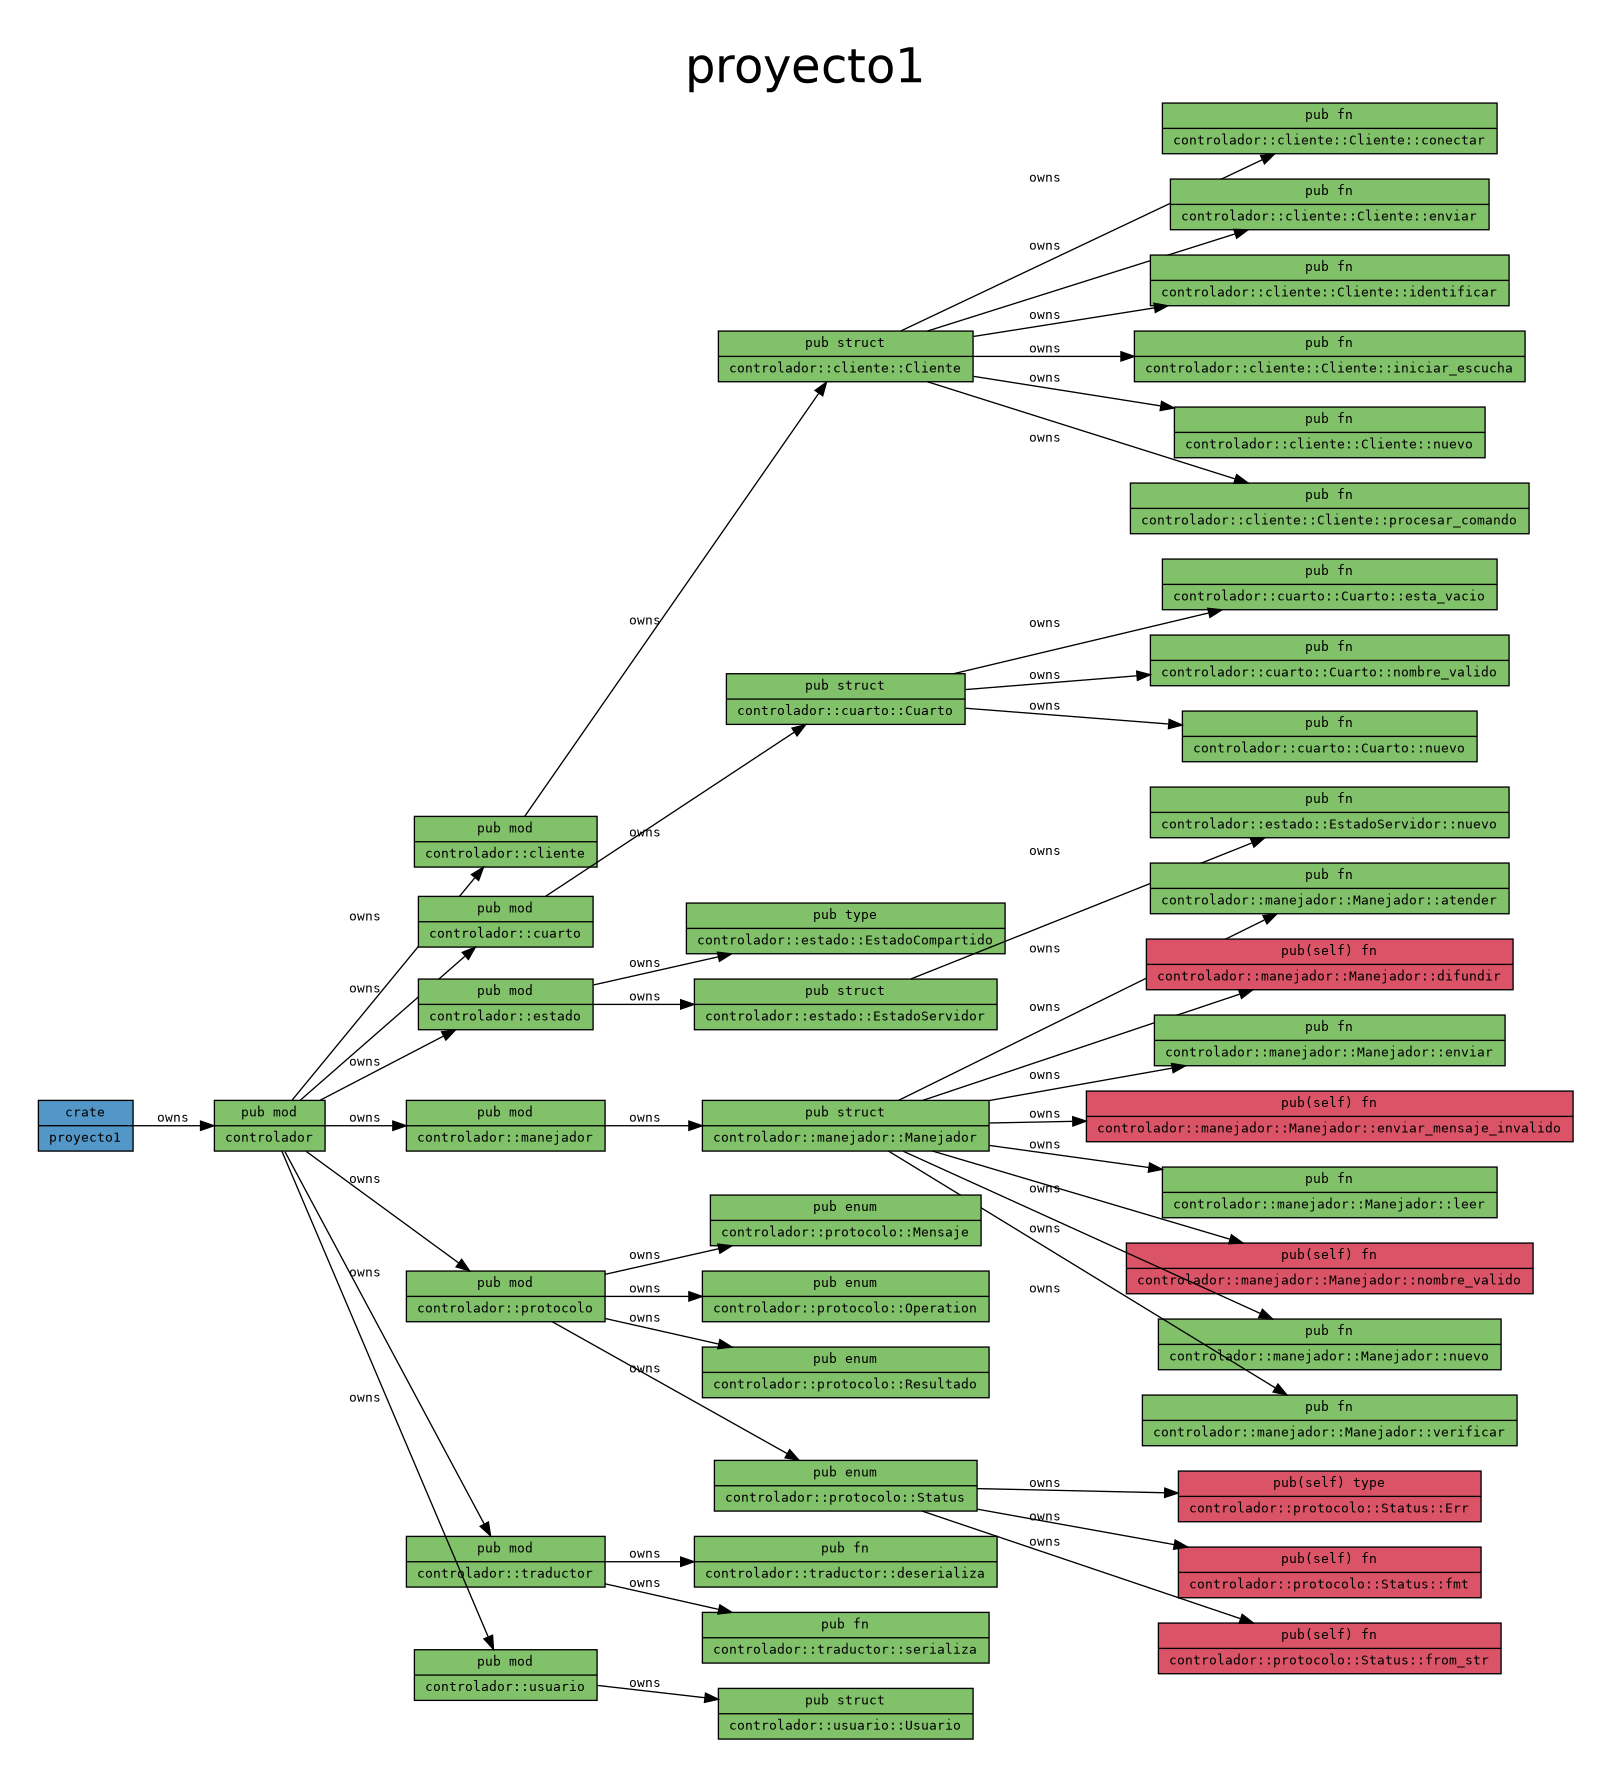
\includegraphics[width=\textwidth]{controlador.png}
    \caption{UML del controlador}
    \label{fig:modulos}
\end{figure}

\begin{figure}[H]
    \centering
    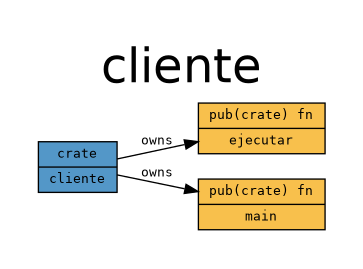
\includegraphics[width=\textwidth]{cliente.png}
    \caption{UML del cliente}
    \label{fig:modulos}
\end{figure}

\begin{figure}[H]
    \centering
    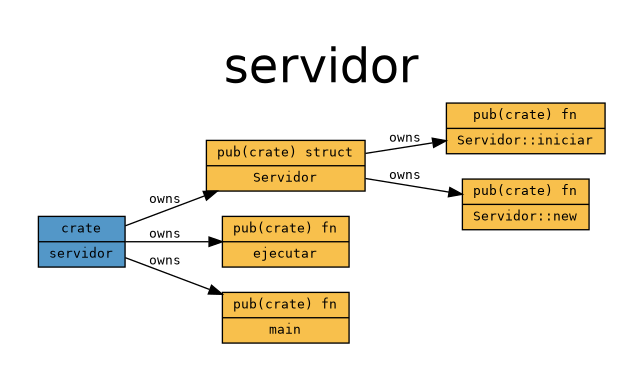
\includegraphics[width=\textwidth]{servidor.png}
    \caption{UML del servidor}
    \label{fig:modulos}
\end{figure}

\section*{Conclusiones}

Realizar este proyecto fue bastante formativo, pensar en el análisis y diseño del mismo, aprender un nuevo lenguaje para implementar la solución y utilizar herramientas para hacerlo parte del software libre fue una tarea bastante ardua.\\

Cada parte del desarrollo fue importante y si hubieramos evitado alguna quizá no lo podríamos haber concluído. Incluso este mismo reporte nos resultó importante al explicar a otros que fue lo que hicimos para contruir nuestro chat.\\

Las herramientas que usamos en este proceso, fueron nuevas para nosotros. Y resultaron ser muy enriquecedoras para contruir este proyecto. Es muy seguro que las volvamos a usar para futuro proyectos junto a otras que aparezcan al resolver problemas en el futuro.\\

Y el aprendizaje más importante que nos llevamos, es el poder resolver problemas por nuestra cuenta. El profesor de la materia nos guío por varios caminos que podíamos seguir para alcanzar la meta, pero al final fuímos nosotros quienes construíos el chat con su ayuda. \\

\nocite{*}
\bibliographystyle{plain}
\bibliography{referencias}

\end{document}

